% !TeX root = ../main.tex

\chapter{算法实现与比较}

亏格测试数据采用 Blender 软件生成,通过 Cube 模型的布尔修改器得到,并导出为 obj 格式。实现代码均位于 \url{https://github.com/libreliu/GeoProcessing}。

GIM 算法和计算最短同调圈的算法均采用 Python 语言编写,使用 OpenMesh 处理网格,并采用 PyVista 进行网格可视化。

图 \ref{fig:genus2him} 展示了计算最短同调圈算法对亏格为 2 的立方体的输出。

\begin{figure}[h]
    \centering
    \begin{subfigure}{.2\textwidth}
        \centering
        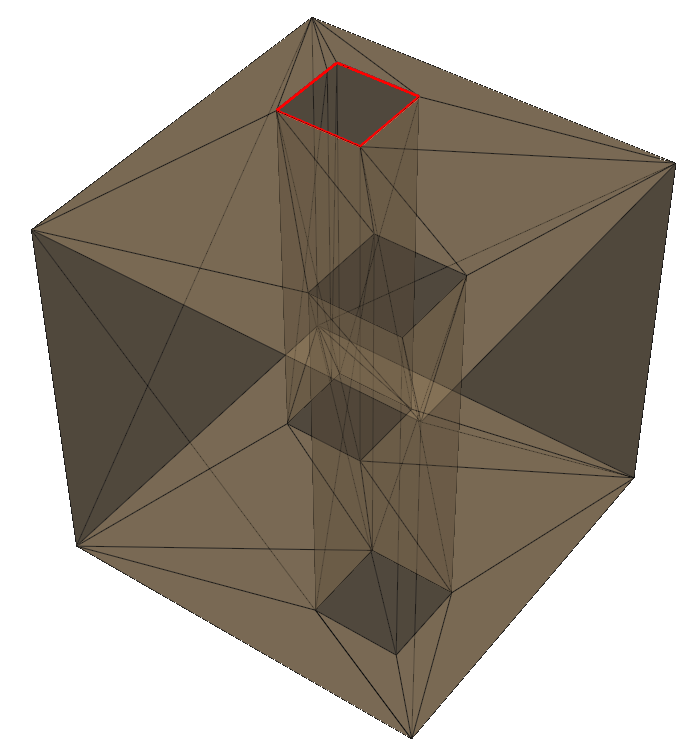
\includegraphics[width=\textwidth]{Genus2_0_optim.png}
        % \caption{提取经纬线前}
    \end{subfigure}
    \begin{subfigure}{.2\textwidth}
        \centering
        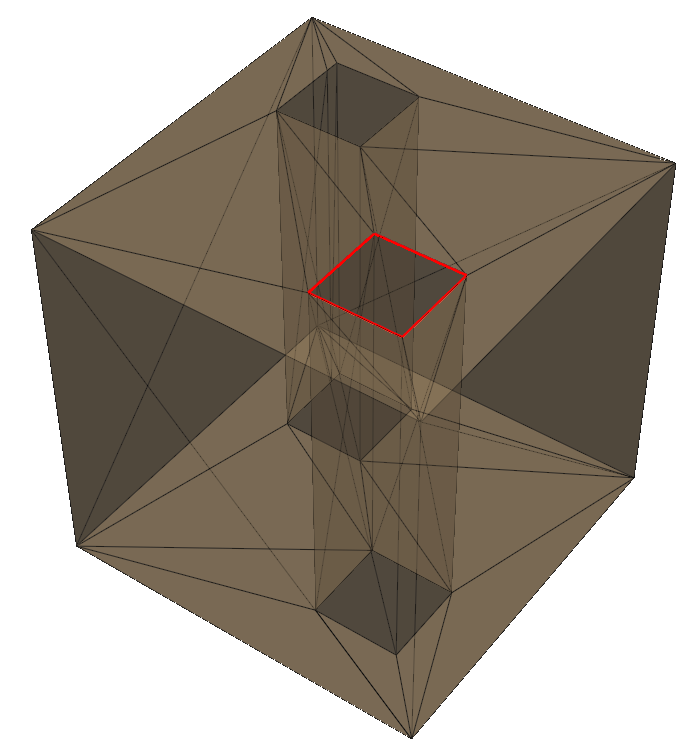
\includegraphics[width=\textwidth]{Genus2_1_optim.png}
        % \caption{提取经纬线后}
    \end{subfigure}
    \begin{subfigure}{.2\textwidth}
        \centering
        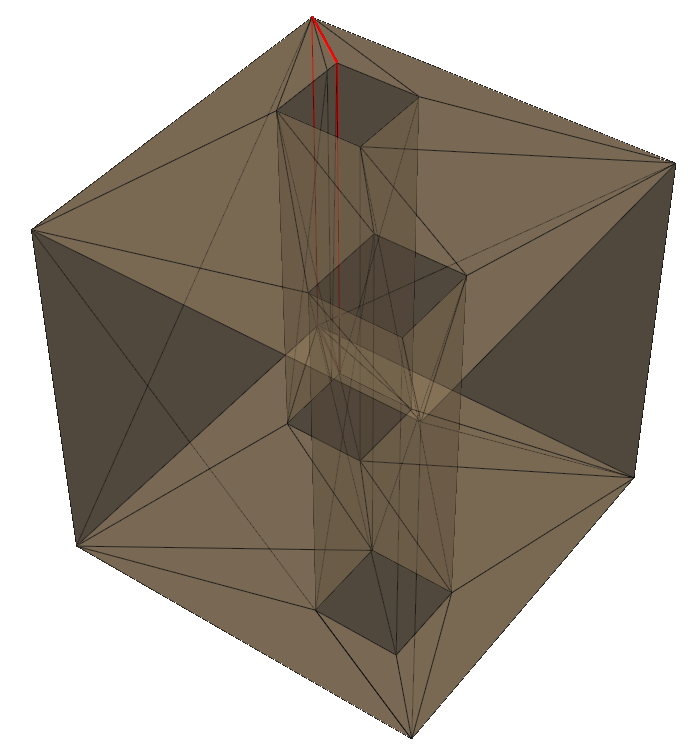
\includegraphics[width=\textwidth]{Genus2_2_optim.png}
        % \caption{提取经纬线后}
    \end{subfigure}
    \begin{subfigure}{.2\textwidth}
        \centering
        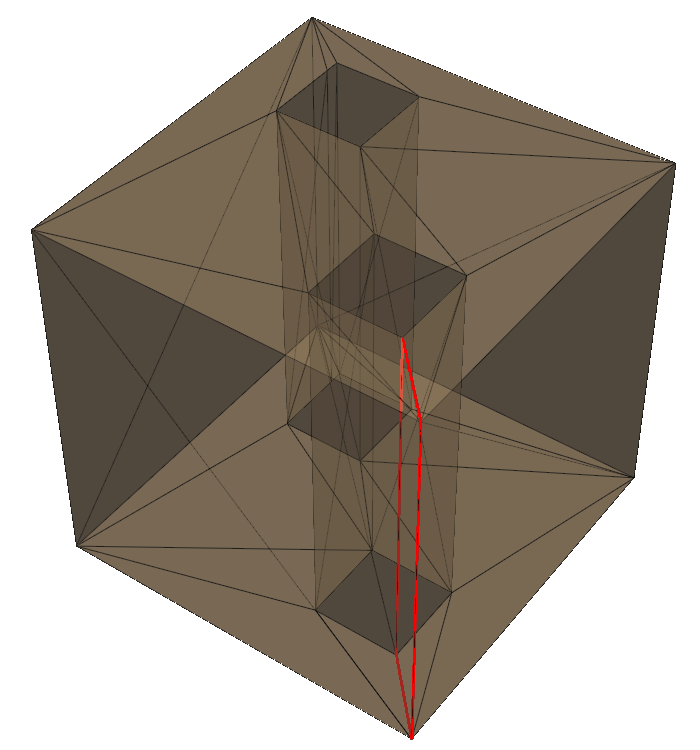
\includegraphics[width=\textwidth]{Genus2_3_optim.png}
        % \caption{提取经纬线后}
    \end{subfigure}
    \caption{亏格为 2 模型的最短同调圈}
    \note{红色为同调基圈,共 4 个}
    \label{fig:genus2him}
\end{figure}

图 \ref{fig:eighthim} 展示了计算最短同调圈算法对亏格为 2 的 2-环面的输出。

\begin{figure}[h]
    \centering
    \begin{subfigure}{.2\textwidth}
        \centering
        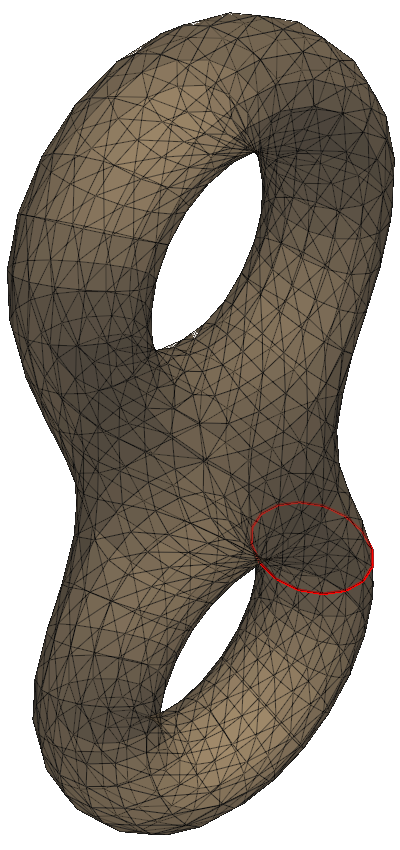
\includegraphics[width=\textwidth]{eight_0_optim.png}
        % \caption{提取经纬线前}
    \end{subfigure}
    \begin{subfigure}{.2\textwidth}
        \centering
        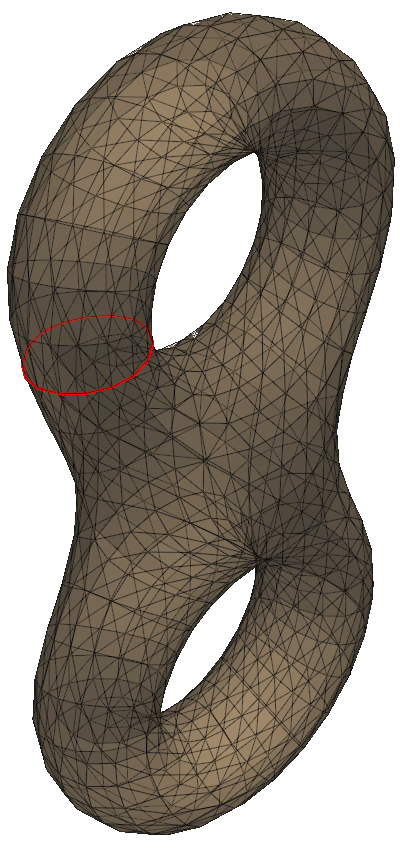
\includegraphics[width=\textwidth]{eight_1_optim.png}
        % \caption{提取经纬线后}
    \end{subfigure}
    \begin{subfigure}{.2\textwidth}
        \centering
        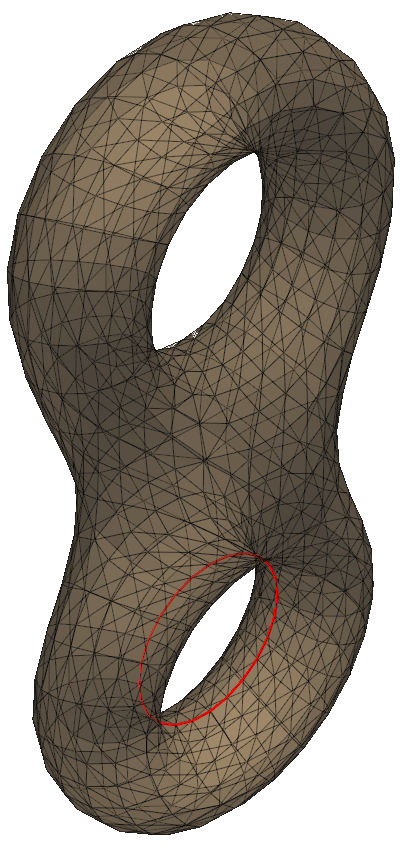
\includegraphics[width=\textwidth]{eight_2_optim.png}
        % \caption{提取经纬线后}
    \end{subfigure}
    \begin{subfigure}{.2\textwidth}
        \centering
        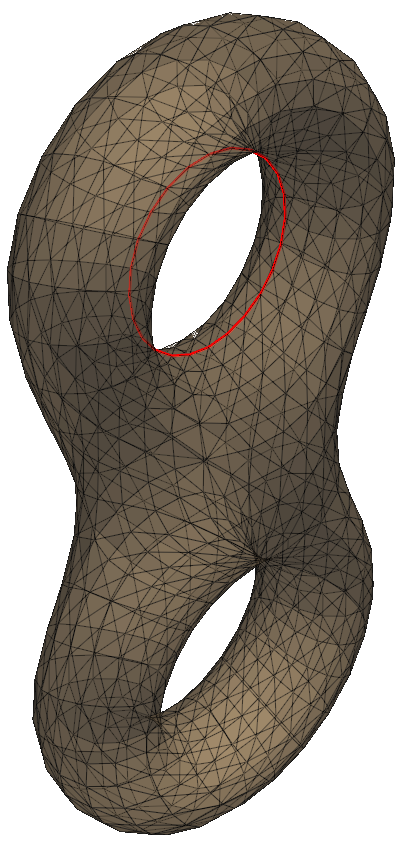
\includegraphics[width=\textwidth]{eight_3_optim.png}
        % \caption{提取经纬线后}
    \end{subfigure}
    \caption{亏格为 2 模型的最短同调圈}
    \note{红色为同调基圈,共 4 个}
    \label{fig:eighthim}
\end{figure}

可以看到,最短同调圈计算的实现是正确的。